\section{Problem}

As found in \cite{g:gridworld}, let there be a grid with five static obstacles (O) in which a robot needs to find the exit (F). The robot can only observe whether the current position is a trap or an exit when moving. The initial state of the robot is also uncertain, it has four possible initial positions (P). The size of the grid $N$ determines the actual positions of the obstacles and the possible initial positions of the robot. The exit will remain static in the north-east. The robot is allowed to move north, east, south or west. The robot also has a probability of $0.1$ of slipping. When the robot slips it will move two tiles at once, when possible. If the robot will encounter a border, it will not move past the border but simply stop there.

In \figureref{f:n5grid} we have the view of the grid for $N=5$ and in \figureref{f:n10grid} we see the grid for $N=10$.

\begin{figure}[H]

\begin{subfigure}[H]{0.45\textwidth}
	\centering
\begin{tikzpicture}[cell/.style={rectangle,draw}]
  \matrix[
  matrix of nodes,
  execute at begin cell=\strut,
  execute at empty cell={\node{\strut};},
  nodes={cell,anchor=center,minimum width=1cm, minimum height=1cm}]{
&  &  &  & F \\
& O.P & P & O & O \\
&  &  &  &  \\
& P & P & & O\\
& O &  &  & \\};
\end{tikzpicture}
\caption{$N=5$}
\label{f:n5grid}
\end{subfigure}
\hfill
\begin{subfigure}[H]{0.45\textwidth}
\centering
\begin{tikzpicture}[cell/.style={rectangle,draw}]
  \matrix[
  matrix of nodes,
  execute at begin cell=\strut,
  execute at empty cell={\node{\strut};},
  nodes={cell,anchor=center,minimum width=0.75cm,minimum height=0.75cm}]{
& & & & & & & & & F\\
& & & & & &O & P & O & \\
& & & & & & & & & O \\
& & & & & & & & &  \\
& & & & & & & & &  \\
& & & & & & & & &  \\
& & & & & & & & &  \\
& P & & & & & & & &  \\
& P & P & & & & & & & O \\
& O & & & & & & & & \\};
\end{tikzpicture}
\caption{$N=10$}
\end{subfigure}
\label{f:n10grid}
\caption{Grid overview for given $N$}
\label{f:examples_case_study}
\end{figure}

The robot has a possibile of observing four different observations.
\begin{enumerate}
\item \texttt{start}: the robot is in the start position.
\item \texttt{traps}: the robot has encountered an obstacle.
\item \texttt{notbad}: the robot has encountered nothing of interest.
\item \texttt{goal}: the robot has reached the final position.
\end{enumerate} 

Let us look at a specific history-based reward function for this grid. If the robot before reaching the exit encounters
\begin{itemize}
\item no obstacles, the reward is 100.
\item one obstacle, the reward is 50.
\item two obstacles, the reward is 25.
\item move than three, the reward is zero.
\end{itemize}

\towrite{This figure needs to be reworked}
These requirements can be transformed into five regular expressions. When combining them together with their respective rewards, we can create a reward controller as seen in \figureref{f:rc_gridworld}

\begin{figure}[H]
	\centering
		\begin{tikzpicture}[node distance=3cm,on grid,auto]
			\node[initial,state] (1) 			{$q_0/100$};
			\node[state] (2) [right=of 1]		{$q_1/50$};
			\node[state] (3) [right=of 2]		{$q_2/25$};
			\node[state] (4) [right=of 3]		{$q_3/10$};
			\node[state] (5) [right=of 4]		{$q_4/0$};
			\path[->] 	(1) edge[loop above] 	node [above,text width=1.5cm,align=center] {\texttt{start, notbad, goal}}			()
							edge[] 	node [above] {\texttt{traps}}			(2)
						(2) edge[loop above] 	node [above,text width=1.5cm,align=center] {\texttt{start, notbad, goal}}			()
							edge[] 	node [above] {\texttt{traps}}			(3)
						(3) edge[loop above] 	node [above,text width=1.5cm,align=center] {\texttt{start, notbad, goal}}			()
							edge[] 	node [above] {\texttt{traps}}			(4)
						(4) edge[loop above] 	node [above,text width=1.5cm,align=center] {\texttt{start, notbad, goal}}			()
							edge[] 	node [above] {\texttt{traps}}			(5)
						(5) edge[loop above] node [above,text width=1.5cm,align=center] {\texttt{start, notbad, goal, traps}}			();
	\end{tikzpicture}
\caption{Reward Controller for given requirements}
	\label{f:rc_gridworld}
\end{figure}

The goal for this situation is to find a policy that maximizes the expected reward given a maximum observation sequence $T$.

\section{Results}
For testing this scenario, we have to pick the maximum observation sequence length $T$ as we have seen in \defref{d:limited_pomdp}. 
We have run the benchmark toolchain for creating policies for POMDPs\cite{g:toolchain} on a system which runs on \texttt{Ubuntu 20.04.3 LTS}. The system has a \texttt{Intel Core i3-6006U} processor and 4GB of RAM.

This tool solves the POMDP given a specific property that we want to check. For our problem we want to find the maximum expected reward after reading a sequence up to length $T$, given the reward function as stated above. The tool finds this value and then finds a policy that complies with this value. A pMC will be generated for finding an optimal policy. The size of this is represented in number of states and number of transitions. 

The empty slots depict the fact that the size of the pMC was too big to be solved. \todo{move tables to appendix?}
\begin{sidewaystable}
\centering
\begin{tabular}{|r|c|c|c|c|c|c|c|c|c|c|}
\hline
T & 50 & 100 & 150 & 200 & 250 & 300 & 350 & 400 & 450 & 500 \\ \hline
Solver time (s) & 2.28 & 6.68 & 11.96 & 18.77 & 26.62 & 35.84 & 46.69 & 58.40 & 71.42 & - \\
Encoding time (s) & 148.55 & 364.16 & 525.13 & 695.75 & 880.37 & 1055.46 & 1242.38 & 1422.13 & 1603.73 & - \\
\# pMC states & 32432 & 73532 & 114632 & 155732 & 196832 & 237932 & 279032 & 320132 & 361232 & 402332 \\
\# pMC transitions & 63222 & 143442 & 223662 & 303882 & 384102 & 464322 & 544542 & 624762 & 704982 & 785202 \\
Result & 0.22608 & 0.22625 & 0.22625 & 0.22625 & 0.22625 & 0.22625 & 0.22625 & 0.22625 & 0.22625 & 0.22625 \\	 \hline
\end{tabular}
\caption{Results for $N=5$}


\vspace{2\baselineskip}
\begin{tabular}{|r|c|c|c|c|c|c|c|c|c|c|}
\hline
T & 5 & 10 & 15 & 20 & 25 & 30 & 35 & 40 & 45 & 50\\ \hline
Solver time (s) & 0.16 & 2.95 & 8.21 & 15.11 & 24.17 & 35.22 & 49.19 & 61.07 & 77.37 & - \\
Encoding time (s) & 
11.95 & 172.79 & 383.88 & 595.19 & 805.52 & 1025.71 & 1232.19 & 1425.90 & 1638.00 & - \\
\# pMC states & 2740 & 39908 & 88268 & 136628 & 184988 & 233348 & 281708 & 330068 & 378428 & 426788 \\
\# pMC transitions & 5223 & 77819 & 172564 & 267309 & 362054 & 456799 & 551544 & 646289 & 741034 & 835779 \\
Result & 
0.034790 & 0.20539 & 0.21518 & 0.21620 & 0.21636 & 0.21639 & 0.21640 & 0.21640 & 0.21640 & 0.21640 \\ \hline
\end{tabular}
\caption{Results for $N=10$}

\end{sidewaystable}


\begin{figure}[H]
\centering
\begin{subfigure}[H]{0.4\textwidth}
	\centering

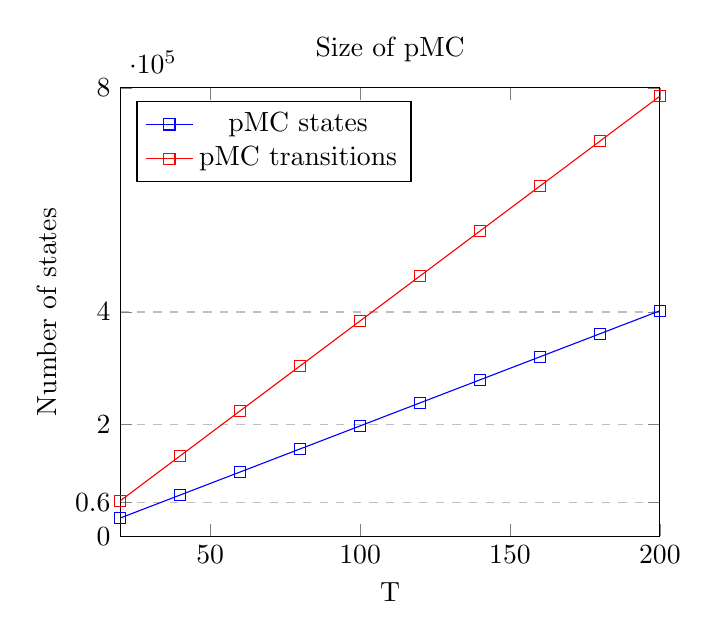
\begin{tikzpicture}
\begin{axis}[
    title={Size of pMC},
    xlabel={T},
    ylabel={Number of states},
    xmin=20, xmax=200,
    ymin=0, ymax=800000,
    xtick={0,50,100,150,200},
    ytick={0,200000,400000,60000,800000},
    legend pos=north west,
    ymajorgrids=true,
    grid style=dashed,
]

\addplot[
    color=blue,
    mark=square,
    ]
    coordinates {
    (20,32432)(40,73532)(60,114632)(80,155732)(100,196832)(120,237932)(140,279032)(160,320132)(180,361232)(200,402332)
    };
    
\addplot[
    color=red,
    mark=square,
    ]
    coordinates {
    (20,63222)(40,143442)(60,223662)(80,303882)(100,384102)(120,464322)(140,544542)(160,624762)(180,704982)(200,785202)
    };
    \legend{pMC states, pMC transitions}

\end{axis}
\end{tikzpicture}
\end{subfigure}
\hfill
\begin{subfigure}[H]{0.4\textwidth}
	\centering
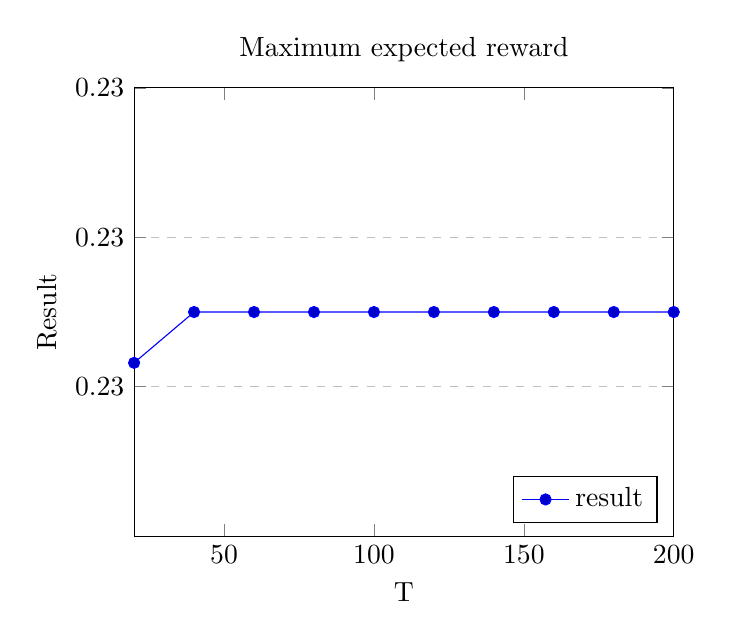
\begin{tikzpicture}

\begin{axis}[
    title={Maximum expected reward},
    xlabel={T},
    ylabel={Result},
    xmin=20, xmax=200,
    ymin=0.2255,ymax=0.227,
    xtick={0,50,100,150,200},
    ytick={0.226,0.2265,0.227},
    legend pos=south east,
    ymajorgrids=true,
    grid style=dashed]    
\addplot
    coordinates {
    (20,0.22608)(40,0.22625)(60,0.22625)(80,0.22625)(100,0.22625)(120,0.22625)(140,0.22625)(160,0.22625)(180,0.22625)(200,0.22625)
    };
    \legend{result}
    
\end{axis}
\end{tikzpicture}
\end{subfigure}

\begin{subfigure}[H]{0.4\textwidth}
	\centering
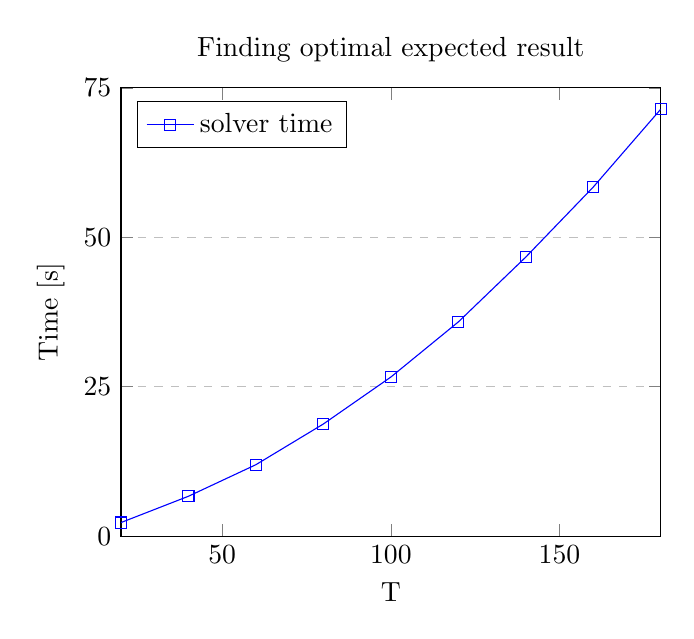
\begin{tikzpicture}
\begin{axis}[
    title={Finding optimal expected result},
    xlabel={T},
    ylabel={Time [s]},
    xmin=20, xmax=180,
    ymin=0, ymax=75,
    xtick={0,50,100,150,200},
    ytick={0,25,50,75},
    legend pos=north west,
    ymajorgrids=true,
    grid style=dashed,
]

\addplot[
    color=blue,
    mark=square,
    ]
    coordinates {
    (20,2.28)(40,6.68)(60,11.96)(80,18.77)(100,26.62)(120,35.84)(140,46.69)(160,58.40)(180,71.42)
    };
    \legend{solver time}

\end{axis}
\end{tikzpicture}
\end{subfigure}
\hfill
\begin{subfigure}[H]{0.4\textwidth}
	\centering
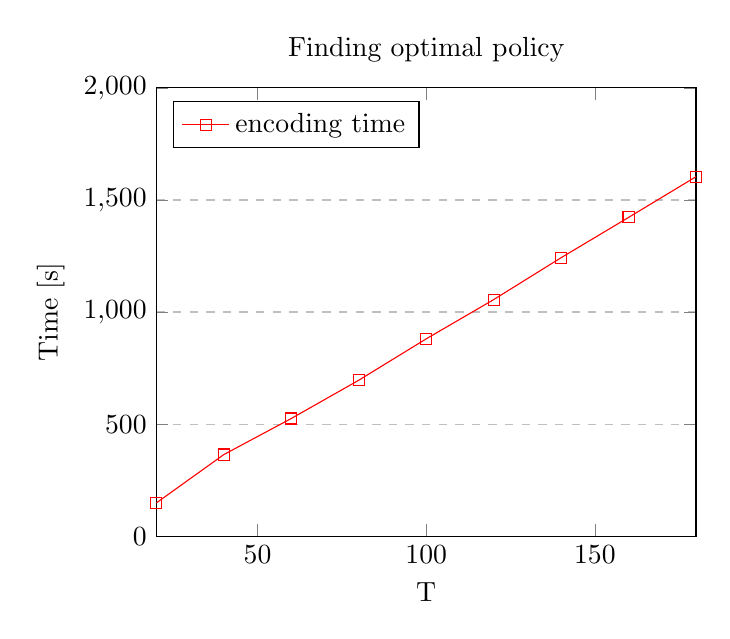
\begin{tikzpicture}
\begin{axis}[
    title={Finding optimal policy},
    xlabel={T},
    ylabel={Time [s]},
    xmin=20, xmax=180,
    ymin=0, ymax=2000,
    xtick={0,50,100,150},
    ytick={0,500,1000,1500,2000},
    legend pos=north west,
    ymajorgrids=true,
    grid style=dashed,
]
    
\addplot[
    color=red,
    mark=square,
    ]
    coordinates {
    (20,148.55)(40,364.16)(60,525.13)(80,695.75)(100,880.37)(120,1055.46)(140,1242.38)(160,1422.13)(180,1603.73)
    };
    \legend{encoding time}
    
\end{axis}
\end{tikzpicture}
\end{subfigure}
\caption{Results for $N=5$}
\end{figure}









\begin{figure}[H]
\centering
\begin{subfigure}[H]{0.4\textwidth}
	\centering

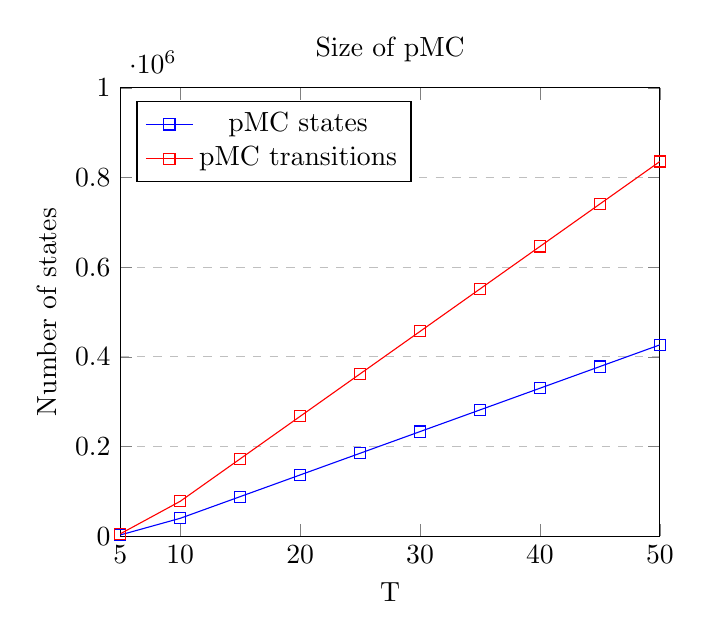
\begin{tikzpicture}
\begin{axis}[
    title={Size of pMC},
    xlabel={T},
    ylabel={Number of states},
    xmin=5, xmax=50,
    ymin=0, ymax=1000000,
    xtick={5,10,20,30,40,50},
    ytick={0,200000,400000,600000,800000,1000000},
    legend pos=north west,
    ymajorgrids=true,
    grid style=dashed,
]

\addplot[
    color=blue,
    mark=square,
    ]
    coordinates {
(5,2740)(10,39908)(15,88268)(20,136628)(25,184988)(30,233348)(35,281708)(40,330068)(45,378428)(50,426788)
    };
    
\addplot[
    color=red,
    mark=square,
    ]
    coordinates {
(5,5223)(10,77819)(15,172564)(20,267309)(25,362054)(30,456799)(35,551544)(40,646289)(45,741034)(50,835779)
    };
    \legend{pMC states, pMC transitions}
    
\end{axis}
\end{tikzpicture}
\end{subfigure}
\hfill
\begin{subfigure}[H]{0.4\textwidth}
	\centering
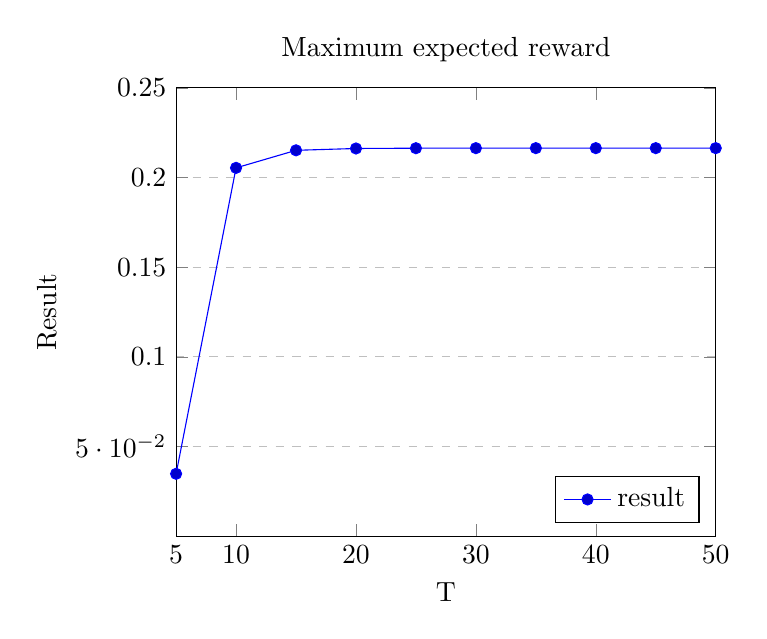
\begin{tikzpicture}

\begin{axis}[
    title={Maximum expected reward},
    xlabel={T},
    ylabel={Result},
    xmin=5, xmax=50,
    ymin=0, ymax=0.25,
    xtick={5,10,20,30,40,50},
    ytick={0.05,0.1,0.15,0.2,0.25},
    legend pos=south east,
    ymajorgrids=true,
    grid style=dashed,
]
    
\addplot
    coordinates {
(5,0.034790)(10,0.20539)(15,0.21518)(20,0.21620)(25,0.21636)(30,0.21639)(35,0.21640)(40,0.21640)(45,0.21640)(50,0.21640)
    };
    \legend{result}
    
\end{axis}
\end{tikzpicture}
\end{subfigure}

\begin{subfigure}[H]{0.4\textwidth}
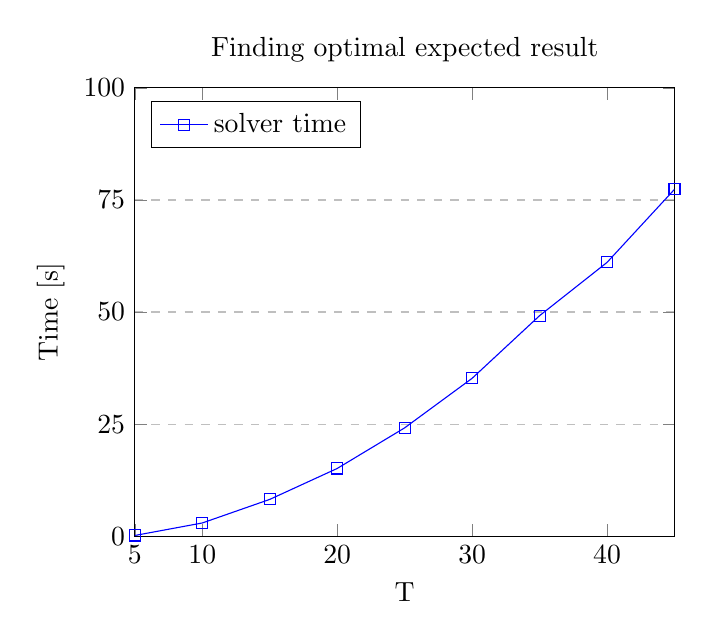
\begin{tikzpicture}
\begin{axis}[
	title={Finding optimal expected result},
    xlabel={T},
    ylabel={Time [s]},
    xmin=5, xmax=45,
    ymin=0, ymax=100,
    xtick={5,10,20,30,40,50},
    ytick={0,25,50,75,100},
    legend pos=north west,
    ymajorgrids=true,
    grid style=dashed,
]

\addplot[
    color=blue,
    mark=square,
    ]
    coordinates {
(5,0.16)(10,2.95)(15,8.21)(20,15.11)(25,24.17)(30,35.22)(35,49.19)(40,61.07)(45,77.37)
    };
    \legend{solver time}
    
\end{axis}
\end{tikzpicture}
\end{subfigure}
\hfill
\begin{subfigure}[H]{0.4\textwidth}
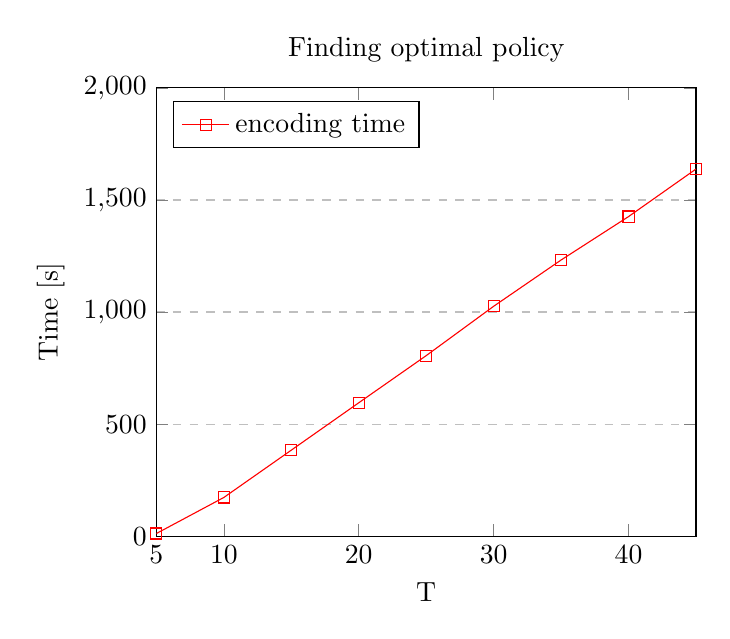
\begin{tikzpicture}
\begin{axis}[
title={Finding optimal policy},
    xlabel={T},
    ylabel={Time [s]},
    xmin=5, xmax=45,
    ymin=0, ymax=2000,
    xtick={5,10,20,30,40,50},
    ytick={0,500,1000,1500,2000},
    legend pos=north west,
    ymajorgrids=true,
    grid style=dashed,
]
    
\addplot[
    color=red,
    mark=square,
    ]
    coordinates {
(5,11.95)(10,172.79)(15,383.88)(20,595.19)(25,805.52)(30,1025.71)(35,1232.19)(40,1425.90)(45,1638.00)
    };
    \legend{encoding time}
    
\end{axis}
\end{tikzpicture}
\end{subfigure}
\caption{Results for $N=10$}
\end{figure}
For $N=5$ we observe that the maximum expected reward had been reached already when $T=50$.

For $N=10$ we can see that the maximum expected reward has been reached for when $T=35$. This can be decreased if we allow for a certain error margin.

The sizing of the pMC that is needed to solve for the policy for optaining the maximum expected reward seems to be linear, in terms of states as wel ass transitions. Since the solver for finding the optimal expected reward is a bit more than linear, it would be pertinent to find the smallest $T$ possible, given a certain error margin for the expected maximum reward.
